\settitle[CorkaMIX]{CorkaMIX : création d'un polyglotte binaire}


\setauthor[M.~Albertini]{Ange Albertini\\
  \email{ange.albertini@gmail.com}}

%\institute{Corkami}

\maketitle
\index{Ange, M.}

\begin{abstract}
	De l'exploitation à l'infection, les {\it malwares} modernes utilisent de nombreux formats de fichier binaires.
        Il est crucial de pouvoir correctement les identifier et les analyser, si possible de manière automatique.
        À priori clairement différenciés, il est malheureusement possible de combiner certains d'entre eux dans un seul et même fichier.
        À des fins de démonstration, un tel binaire {\it polyglotte} a été crée, en incluant plusieurs caractéristiques non documentées de chaque format concerné.
\end{abstract}


\section{Introduction}

\subsection{État de l'art}

Un fichier polyglotte est un seul et meme fichier fonctionnant comme on s'y attend avec plusieurs languages differents.  Un des plus simple d'entre eux, représenté David Kendall Polyglot figure~\ref{lst:albertini:polyglot}, fonctionne en Ruby, Perl, PHP, ksh, Scheme, Lisp, Clojure, Plan. Les {\it polyglottes} peuvent aller beaucoup plus loin, jouant sur les différences d'interprétation et de {\it pré-processing} de chaque language inclu.

\begin{lstlisting}[language={},caption={un programme polyglotte simple},label={lst:albertini:polyglot}]
 (print "Hello, world!\n");
\end{lstlisting}
Cependant, les formats de fichiers binaires sont, eux, rarement compatible, car exclusifs: en effet, la majeure partie d'entre eux doivent nécessairement débuter par une {\it signature} dite 'nombre magique', à chaque fois différente, à de rares exceptions près (tel que CAFEBABE pour le format Mach-O universel et les classes JAVA).

Il ne semble donc pas possible de combiner des formats binaires en général. Cependant, il y a quelques exceptions. Et hélàs - ce n'est pas une coincidence - il s'agit des formats parmi les plus utilisés ces dernières années pour la prolifération de {\it malware}.

\subsection{Pivot}

Le format pivot de la grande majeure partie des virus est le format de binaire universel de Windows, appelé le format {\it Portable Executable}, ou {\em PE}. Pour ce rôle unique dans la chaîne virale, il a donc été choisi comme point de départ.

\section{exploration du format {\em PE}}
Ce format stipule que le fichier commence par une structure {\em IMAGE\_DOS\_HEADER}, de 40 octets:
\begin{itemize}
\item les 2 premiers octets de cette structure, appelé {\em e\_magic}, contiennent obligatoirement la signature {\em MZ} (bien que le vieux format d'exécutable DOS tolérait officieusement les lettres {\em ZM} - probablement à titre comique - ce n'est plus le cas pour les fichiers {\em PE}. Il est donc impossible de le combiner à tout autre format imposant une signature spécifique à l'octet 0.
\item tous les champs suivants, à l'exception du dernier, ne concerne que la fonctionnalité DOS de l'exécutable - qui se borne en majeure partie à afficher un message d'erreur, elle est totalement ignorée quand le fichier est chargé en tant que {\em PE}.
\item le dernier champ, {\em e\_lfanew}, est un pointeur sur 32 bits vers la structure suivante de l'exécutable
\end{itemize}

On sait donc que notre fichier doit commencer par {\em M} et {\em Z}, et qu'au déplacement $0x3C$ doit se trouver un pointeur. Entre les deux, on peut y faire ce que l'on veut, tout en gardant la fonctionalité {\em PE} intacte.

C'est ce que nous allons faire en y intégrant un script Python.

\subsection{intégration d'un script Python}

un script Python est un fichier texte qui commence à l'octet 0. les 2 premières lettres étant imposées, il faut donc utiliser ce {\em MZ} en créant, par exemple, une variable fictive.
\begin{lstlisting}[language={Python},caption={un script python commençant par MZ},label={lst:albertini:pythonMZ}]
MZ=1
\end{lstlisting}

Mais l'interpréteur Python vérifie à l'avance l'encodage de tout le fichier source. Sachant que la structure suivante, pointée par {\em e\_lfanew}, {\em IMAGE\_NT\_HEADERS} a comme premier champ {\em Signature} qui doit contenir les caractères nuls, on se trouve face à un obstacle.

Il est néanmoins facile à contourner, il suffit d'insérer entre le déplacement 0 et cette {\em Signature} un caractère de fin de fichier, {\em EOF}, dont le code est 26.

On a aussi la place d'insérer une partie de script Python fonctionnelle, histoire de prouver que ça marche effectivement.
Le python ne permettant pas lui-même de générer un caractère de fin de fichier dans son propre source (sans quoi, logiquement, le fichier sera tronqué), le fichier sera nécessairement dorénavant généré en assembleur.
\begin{lstlisting}[language={},caption={un script python généré en assembleur},label={lst:albertini:pythonasm}]
db 'MZ=1;print("Hello World !")'
db 26 ; EOF
\end{lstlisting}

Ça peut se faire avec n'importe quel exécutable, en écrasant l'obsolète {\em IMAGE\_DOS\_HEADER}, à l'exception de sa signature et du dernier champ {\em e\_lfanew}, comme montré à la figure~\ref{fig:albertini:pythonnotepad}.
\begin{figure}[ht]
  \centering
  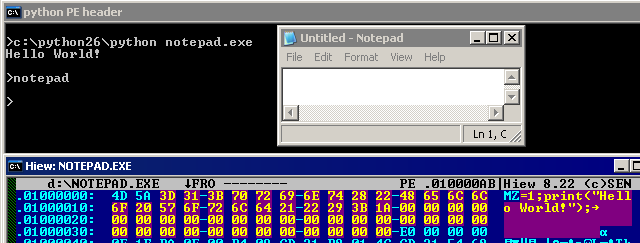
\includegraphics[width=0.8\textwidth]{albertini/img/pythonnotepad}
  \caption{le bloc-note Windows avec un en-tête Python}
  \label{fig:albertini:pythonnotepad}
\end{figure}

\begin{figure}[ht]
  \centering
  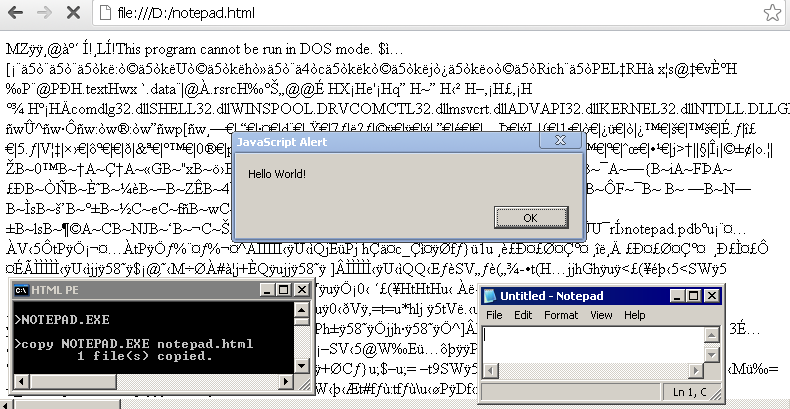
\includegraphics[width=0.8\textwidth]{albertini/img/htmlnotepad}
  \caption{le bloc-note Windows avec une page HTML ajoutée à la fin}
  \label{fig:albertini:pythonnotepad}
\end{figure}

\begin{figure}[ht]
  \centering
  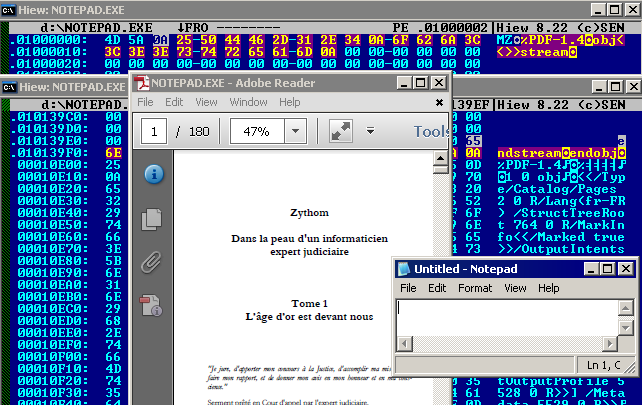
\includegraphics[width=0.8\textwidth]{albertini/img/pdfnotepad}
  \caption{le bloc-note Windows avec un fichier PDF ajouté à la fin}
  \label{fig:albertini:pythonnotepad}
\end{figure}

\bibliography{albertini/biblio}

%%% Local Variables:
%%% mode: TeX-PDF
%%% TeX-master: "master"
%%% End:
